\chapter{Pendolo a torsione}
\section{Introduzione}
\subsection{Oggetto della ricerca}
L'esperienza si prefissa l'obiettivo di misura le costanti di torsione $c$ di tre fili di sezione differente e i momenti d'inerzia di tre oggetti.
\subsection{Metodo}
L'esperienza si compone di tre differenti fasi.
\begin{itemize}
\item Misura sperimentale dello spostamento angolare a seguito del momento della forza peso, al fine di calcolarne il momento d'inerzia 
\item Misura sperimentale del periodo di un pendolo di torsione, al fine di calcolare la costante di torsione dei fili
\item Misura della costante $c$ di torsione tramite l'instaurazione di un equilibrio tra il momento elastico e il momento della forza peso, e confronto con il valore teorico di $c$
\end{itemize}
\subsection{ Strumentazione e dati geometrici}
Nell'esperimento verrà utilizzato un pendolo di torsione strutturato nel seguente modo:
\\
Micrometro: $ \pm 1 \mu m$
 \\
Metro: $\pm 1 mm$
\\
Sensore di rotazione: $\pm 0.09$ gradi
\\

\begin{tabular}{ll}
Masse puntiformi: & 0.074 kg\\
Lunghezza sbarra: & 0.38 m\\
Massa Sbarra: & 0.2563 kg\\
Raggio Sbarra: & 0.0045 m\\
\midrule
Massa anello: & 0.46927 kg\\
Raggio interno: & 0.0265 m\\
Raggio esterno: & 0.0355 m\\
\midrule
Supporto & 0.0035 m\\
\midrule
Massa disco: & 0.12055 kg\\
Raggio disco: & 0.0475 m\\
Diametro carrucola: & 29 mm\\
\end{tabular}

\section{Raccolta dei dati}
Per quanto riguarda i tre fili in esame:
\begin{center}

\begin{tabular}{l|c|c|c|}
 & Filo A & Filo B & Filo C \\
\midrule
Diametro (mm) & 1.750 & 1.175 & 0.880 \\
Lunghezza (cm) & 41.3 &  43 & 33.5 \\
\midrule
\end{tabular}\end{center}

\subsection{Misura dei momenti d'inerzia}

In questa fase si provvederà a ricavare  sperimentalmente i momenti d'inerzia dei seguenti corpi:
\begin{itemize}
\item Disco 
\item Anello
\item Sbarra cilindrica omogenea, con due masse uguali, scorrevoli su di essa, poste equidistanti dall’asse di rotazione (a una distanza di $38\ cm$
\end{itemize}

Si è utilizzato un sistema di due pulleggie e un sensore di rotazione.
Il sensore di rotazione fornisce la posizione angolare in funzione del tempo. 
\\

Acquisiti i dati della posizione angolare in funzione del tempo, è possibile calcolare l'accelerazione angolare del sistema. A questo punto, si può calcolare $I$ nel seguente modo:
$$ bF_p = I\alpha $$
$$ I = \frac{b\cdot mg}{\alpha} $$

\begin{center}
\begin{tabular}{c|ccc}
Oggetto & Accelerazione angolare ($rad/s$) & Momento d'inerzia ($ 10^{-4} \cdot kg\cdot m^2$) \\
\midrule
Anello 60 g&43.05 & 1.983 \\
Anello 75 g &67.48 & 1.581 \\
Anello 100 g&84.43 & 1.685\\
\midrule
Media e $\sigma$&&1.750 $\pm$ 0.209 \\
\midrule
Disco e Anello 60 g&43.05 & 6.637 \\
Disco e Anello 75 g &67.48 & 6.639 \\
Disco e Anello 100 g&84.43 & 6.71\\
Disco e Anello 250 g&43.05 &  6.91 \\
\midrule
Media e $\sigma$&& 6.726 $\pm$ 0.1329\\
\midrule
Sbarra 60 g&43.05 & 50.12\\
Sbarra 100 g &67.48 & 55.78 \\
Sbarra 250 g&84.43 & 56.63\\
\midrule
Media e $\sigma$&& 54.18 $\pm$ 3.539\\
\midrule
\end{tabular}
\end{center}

Per quanto riguarda i momenti d'inerzia \textbf{teorici}:
$$ I_{sbarra} = \frac{1}{2} m R^2 = 84.4\cdot 10^{-4}\ kg\cdot m^2$$
$$ I_{anello} =\frac{1}{2} m (R^2_1 + R^2_2) = 1.3\cdot 10^{-4} \ kg\cdot m^2$$
$$ I_{disco} = \frac{1}{12} m L^2 + 2 \mu D^2 = 4.6\cdot 10^{-4} \ kg \cdot m^2$$



\subsection{Misura dinamica (pendolo di torsione)}

Abbiamo ricavato i seguenti periodi di oscillazione per ogni filo:
\\
\begin{tabular}{cc}
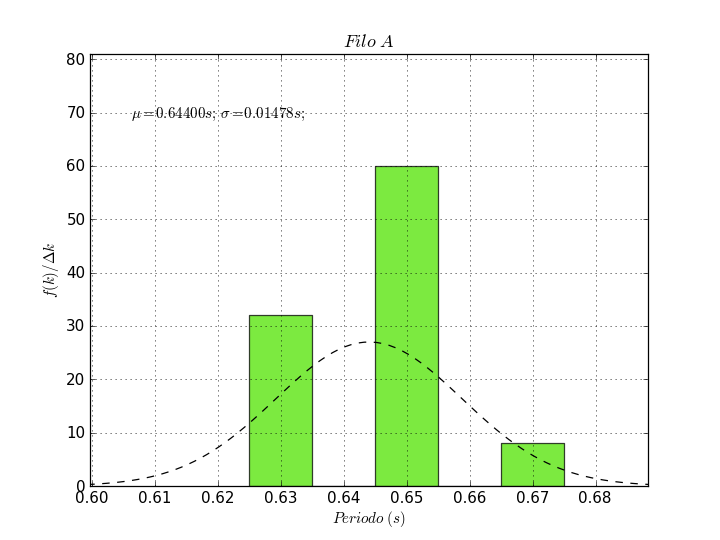
\includegraphics[scale=0.4]{../grafici/FiloA.png}
&
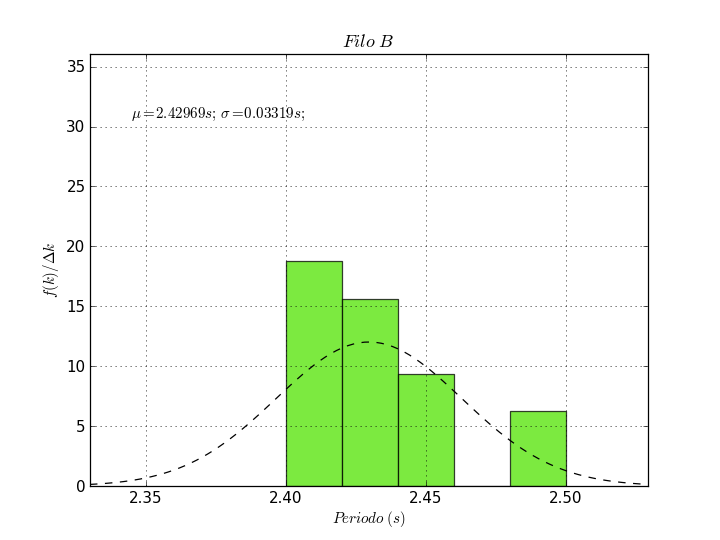
\includegraphics[scale=0.4]{../grafici/FiloB.png}
\\
\begin{tabular}{ll}
Filo A: & $0.644 \pm 0.015\ s$\\
Filo B: & $2.429 \pm 0.033\ s$\\
Filo C: & $3.844 \pm 0.046\ s$
\end{tabular}
&
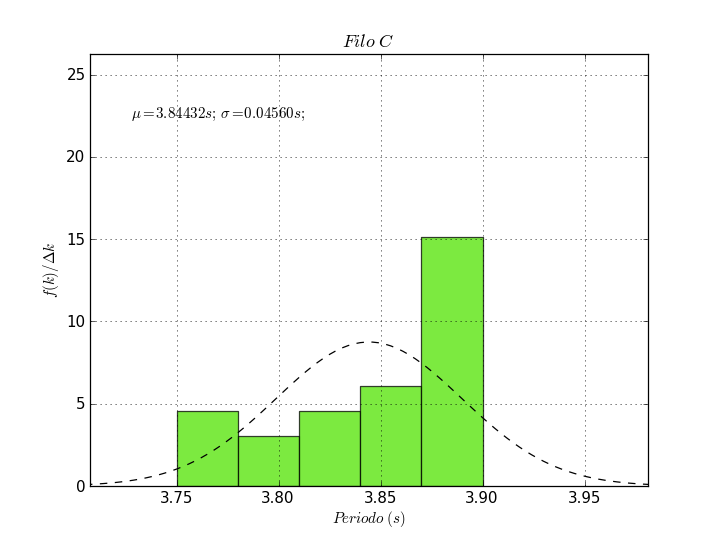
\includegraphics[scale=0.4]{../grafici/FiloC.png}\\

\end{tabular}


Questo ci permette di calcolare la costante di torsione $c$ sfruttando la seguente eguaglianza:
$$ -c\theta = I\frac{d^2\theta}{d\theta^2} $$
che identifica un moto oscillatorio di periodo
$$ T = 2\pi \sqrt{\frac{I}{c}}$$
da cui
$$ c = 4\pi^2\frac{I}{T^2} $$
Riassumendo:

\begin{center}
\begin{tabular}{l||c|c}
& Periodo ($s$) & Costante di torsione ($N\cdot m\cdot rad^{-1}$) \\
\midrule
Filo A: & $0.644 \pm 0.015$ & 95 \\
Filo B: & $2.429 \pm 0.033$ & 6.69\\
Filo C: & $3.844 \pm 0.046$ & 2.67\\
\end{tabular}
\end{center}


\subsection{Misura statica}

Tabulati gli angoli di deflessione per ogni filo in base alla massa sospesa (controlla!)\\
\begin{center}
\begin{tabular}{l|ccc}
& Filo A & Filo B & Filo C \\
\midrule
50g & 4.0 & 12.0 & 31.0 \\
100g & 7.0 & 23.0 & 61.0 \\
200g & 13.0 & 47.0 & 126.0 \\
\midrule
\end{tabular}\end{center}
Essendo il pendolo in equilibrio, poniamo
$$ \tau_{peso} = \tau_{elastico} $$
$$ b\cdot mg = c\theta $$
da cui
$$ c = \frac{b\cdot mg}{\theta} $$
dove $b$ è il braccio di applicazione della forza peso, ovvero il raggio della carrucola.
I valori di $c$ calcolati sono dunque stati (in $N\cdot m\cdot rad^{-1}$):

\begin{center}
\begin{tabular}{l|lll}
Peso & Filo A & Filo B & Filo C \\
\midrule
50g & 0.1019 & 0.0340 & 0.0135 \\
100g & 0.1164 & 0.0354 & 0.0134 \\
200g & 0.1254 & 0.0347 & 0.0129 \\
\midrule
$c_{best}$ & $0.115$ & $0.035$& $0.0137$ \\
$\sigma_{c}$ & $0.012$ & $\sim0$ & $\sim 0$ \\
\end{tabular}
\end{center}

\section{Dipendenza di $c$ da $r^4$}

Per la misura statica di $c$, bisogna utilizzare la seguente relazione:

$$ c = G \frac{\pi}{2}\frac{r^4}{l} $$

dove $G$ è il modulo di rigidità o di scorrimento ed è una proprietà specifica del materiale di cui il filo è realizzato.

Non siamo riusciti a trovare i valori di G tabulati in quanto non conoscevamo il materiale in cui era costruito il filo, quindi abbiamo cercato di arrivare a una migliore stima per riconoscerlo. Abbiamo utilizzato il valore di $c$ misurato in precedenza (misura statica) per calcolare $G$ secondo la seguente formula:

$$ G = \frac{2cl}{\pi r^4} $$

I valori calcolati sono stati:
\begin{center}
\begin{tabular}{lll}
Filo A & Filo B & Filo C \\
\midrule
49 GPa & 78 GPa & 73 GPa \\
\end{tabular}
\end{center}

Da cui abbiamo supposto che il filo A fosse in acciaio, e i fili B e C in titanio.
I dati ufficiali tabulati infatti sono i seguenti:
\begin{center}
\begin{tabular}{ll}
Acciaio & Titanio \\
\midrule
41 GPa & 78 GPa \\
\end{tabular}
\end{center}
Ripetendo il calcolo con G come tabulato, otteniamo:
\begin{center}
\begin{tabular}{lll}
Filo A & Filo B & Filo C \\
\midrule
0.0914 & 0.0339 & 0.0137 \\
\end{tabular}
\end{center}

che è compatibile con i valori misurati in precedenza.

\section{Conclusioni}
Confrontiamo i valori di $c$ teorici e calcolati tramite il metodo statico:
\begin{center}
\begin{tabular}{l|lll}
& Filo A & Filo B & Filo C \\
\midrule
Misura dinamica &  \\
Misura statica & $0.115\ (\pm 0.012)$ & $0.035$& $0.0137$ \\
Misura teorica & 0.0914 & 0.0339 & 0.0137 \\
\midrule
Misura media & 0.103 & 0.03445 & 0.0137\\
Errore ($\sigma_c$) & 0.017 & $\sim 0$ & $\sim 0$\\
\end{tabular}
\end{center}

Per tutti i fili la misurazione statica è ottima, tranne per il filo A, dove la misura è comunque confrontabile. A questo si aggiunge l'incertezza derivante dal non conoscere il materiale di costruzione dei fili.
